\documentclass[12pt]{article}

\usepackage[bottom = 15mm]{geometry}
\usepackage[utf8]{inputenc}
\usepackage[T2A]{fontenc}
\usepackage[russian]{babel}
\usepackage{graphicx}
\usepackage{float}
\usepackage{caption}
\usepackage{amssymb, gensymb, amsmath}
\usepackage{mathrsfs}
\usepackage{array, colortbl}
\usepackage{multicol}


\textwidth = 16 cm
\textheight = 23  cm
\oddsidemargin = 0 pt
\topmargin = -1.5 cm
\parindent = 20 pt
\parskip = 0 pt
\flushbottom


\title{{\bf Задача 4.\,1.\,3 \\ Рефрактометр Аббе}}
\author{Лось Денис (группа 611)}
\date{25 апреля 2018}

\begin{document}

\maketitle

\paragraph*{Цель работы: } знакомство с методом измерения показателей преломления твёрдых и жидких сред в монохроматическом свете.

\paragraph*{В работе используются: } технический рефрактометр Аббе; освети-
тель; набор стеклянных образцов; жидкости с неизвестными показате-
лями преломления (глицерин, этиловый спирт); монобромнафталин;
дистиллированная вода.

\section*{Теоритическая часть: рефрактометрия}
\par
	Показатели преломления жидких и твёрдых тел могут измерять с большой точностью. При данной температуре и для данной длины волны они являются важнейшими постоянными, характеризиющими вещество. Измерения показателей преломления может быть использовано для исследования веществ --- соответствующий разде науки носит название {\bf рефрактомерии}.
\par
	В основе рефрактометрического метода исследования лежит формула Лоренц-Лорентца, связывающая показатель преломления $n$ изотропного вещества с числом молекул $N$ в единице объёма и поляризуемостью $\alpha$ молекул вещества:
\begin{equation}
	\frac{n^2 - 1}{n^2 + 2} = \frac{4 \pi}{3} N \alpha \label{lorlor}
\end{equation}
\par
	Величина
\begin{equation}
	r = \frac{1}{\rho} \, \frac{n^2 - 1}{n^2 + 2},
\end{equation}
	где $\rho$ --- плотность вещества, называется {\bf удельной рефракцией}. Согласно (\ref{lorlor}) удельная рефракция чистого химического вещества зависит только от молекулярных характеристик (массы молекулы $m_0$ и поляризуемости $\alpha$) и равна
\[
	r = \frac{4 \pi}{3} \frac{\alpha}{m_0} = const.
\]
\par
	Предполагая, что оптическое поведение молекул каждого компонента смеси практически не зависит от присутствия других компонентов, можно записать удельную рефракцию смеси веществ через удельные рефракции компонентов и их массовые доли
\begin{equation}
	r = r_1 c_1 + r_2 c_2 + \dots
\end{equation}
\par
	Согласно опыту во многих опытах эмпирическое правило об аддитивности рефракций может быть применено и для рассчёта рефракции сложного химического соединения, если известны рефракции составляющих его элементов.
\par
	Для каждого элемента удобно ввести понятие {\bf атомной рефракции} $R$ как произведения удельной рефракции $r$ на его атомную массу $A$:
\[
	R = A r,
\]
и аналогично для химического соединения --- понятие {\bf молекулярной рефракции} $R_M$:
\begin{equation}
	R_M = M r = \frac{M}{\rho} \, \frac{n^2 - 1}{n^2 + 2} = \frac{4 \pi}{3} \frac{N_A}{\alpha}, \label{MM}
\end{equation}
где $M$ --- молекулярная масса соеднинения, $N_A$ --- постоянная Авогадро.
\par
	Если принять аддитивность молекулярной рефракции, можно записать её как сумму рефракций атомов, составляющих молекулу:
\[
	R_M = q_1 A_1 r_1 + q_2 A_2 r_2 + \dots = q_1 R_1 + q_2 R_2 + \dots ,
\]
где $q_1, q_2, \dots$ --- числа атомов элементов, входящих в состав молекулы.

\section*{Теоритическая часть: рефрактометр Аббе}
\par
	Технический рефрактометр Аббе служит для быстрого (и сравнительно грубого) измерения показетелей преломления жидких и твёрдых тел. 
\par
	Пусть луч света падает на границу раздела двух сред со стороны оптически более плотной среды ($n$ = $n_2$). Для углов падения падения меньших предельного $\varphi_\text{пр}$, свет частично проникает в оптически менее плотную среду ($n$ = $n_1$), и частично отражается. При $\varphi_\text{пр} < \varphi < 90 \degree$ преломлённый луч отсутствует, и наступает полное отражение.
\par
	Предельный угол $\varphi_\text{пр}$ соотвествует углу преломления $90 \degree$, следовательно,
\[
	\sin\varphi_\text{пр} = \frac{n_1}{n_2}.
\]
	Зная показатель преломления одной из сред и определяя на опыте предельный луч, можно найти показатель преломления второй среды.
\par
	Пусть свет падает на границу раздела со стороны оптически менее плотной среды. В зависимости от угла падения луч во второй среде может составлять с нормалью углы, расположенные в интервале от нуля до $\varphi_\text{пр}$. Предельный угол преломления $\varphi_\text{пр}$ соответсвует углу падения $90 \degree$.

\paragraph*{Метод скользящего луча}
\par
	Оптическая схема рефрактометра Аббе и ход лучей при измерении показателя преломления жидкости по методу скользящего луча показаны на рис. 1.
	
	\begin{figure}[h!]
		\centering
		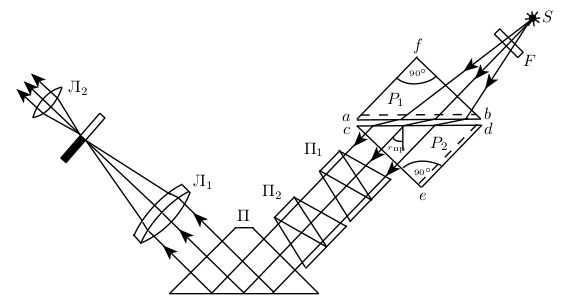
\includegraphics[width = 11cm, height = 5cm]{image1.png}
		\caption{Ход лучей в рефрактометре при измерении показателя преломления жидкости методом скользящего луча}
	\end{figure}
\par
	Основной частью рефрактометра являются две стеклянные прямоугольные призмы $P_1$ и $P_2$, изготовленные из стекла с большим показателем преломления. Свет проникает в призму $P_1$ через грань bf и попадает в жидкость через матовую грань ab. Свет, рассеянный матовой поверхностью, проходит слой жидкости и под всевозможными углами падает на
грань cd призмы $P_2$.
\par
	Если свет, выходящий из грани ce, пропустить через собирающую линзу Л1 , то в её фокальной плоскости наблюдается резкая граница света и темноты. Граница рассматривается с помощью линзы Л2. Линзы Л1 и Л2 образуют зрительную трубу, установленную на бесконечность.
В их общей фокальной плоскости находится изображение шкалы величин показателя преломления и указатели (нить и перекрестие). В поле зрения окуляра Л2 трубы одновременно можно увидеть только часть изображения шкалы и часть поля сфокусированных лучей, выходящих из призмы P2 . Вращая систему призм P1 и P2 и, следовательно, изменяя наклон предельного пучка лучей относительно оси зрительной трубы, можно добиться, чтобы граница света и тени оказалась в поле зрения окуляра Л2 и совпала с положением указателя. Значение показателя преломления жидкости отсчитывается по шкале на уровне резкой границы света и тени.
\par
	Если источник света S не является монохроматическим, то наблюдаемая в окуляре трубы граница света и темноты часто оказывается размытой и окрашенной из-за дисперсии показателя преломления исследуемого вещества (т. е. из-за зависимости $n$ от длины волны $\lambda$). Для
того чтобы получить и в этом случае резкое изображение границы, на пути лучей, выходящих из призмы P2 , помещают компенсатор с переменной дисперсией. Компенсатор содержит две одинаковые дисперсионные призмы Амичи (призмы П1 и П2), каждая из которых состоит
из трёх склеенных призм, обладающих различными показателями преломления и различной дисперсией. Призмы рассчитываются так, чтобы монохроматический луч с длиной волны $\lambda_D = 589,3$ нм (среднее значение длины волны жёлтого дублета натрия) не испытывал отклонения.
Лучи с другими длинами волн отклоняются в ту или иную сторону.
\par
	Для поворота призм друг относительно друга служат специальная рукоятка и система конических шестерен, с помощью которых призмы одновременно поворачиваются в противоположных направлениях. Вращая ручку компенсатора, следует добиваться того, чтобы граница света и тени в поле зрения стала достаточно резкой. Положение границы при этом соответствует длине волны $\lambda_D$ , для которой обычно и приводятся значения показателя преломления.
\par
	В некоторых случаях, когда дисперсия исследуемого вещества особенно велика, диапазон компенсатора оказывается недостаточным и чёткой границы получить не удаётся. В этом случае стоит устанавливать перед осветителем жёлтый светофильтр.

\paragraph*{Метод полного внутреннего отражения}
\par
	На рис.2 показан ход лучей в рефрактометре при работе по методу полного внутреннего отражения.
	\begin{figure}[h!]
		\centering
		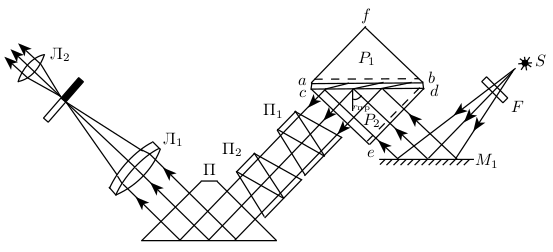
\includegraphics[width = 11cm, height = 5cm]{image2.png}
		\caption{Ход лучей в рефрактометре при измерении показателя преломления жидкости методом полного внутреннего отражения}
	\end{figure}
\par
	В этом случае свет от источника S после отражения от зеркала M1 падает на матовую грань ed призмы P2 (в методе скользящего луча эта поверхность закрывается металлической
шторкой). После рассеяния на грани ed свет падает на границу раздела стекло-жидкость под всевозможными углами. При $r > r_\text{пр}$ наступает полное внутреннее отражение, при $r < r_\text{пр}$ свет отражается частично. В поле зрения трубы наблюдается граница света и полутени.

\section*{Экпериментальная установка: работа с прибором}
\par
	Измерение показателя преломления проводят в следующем порядке. Откинув призму
P1 , с помощью пипетки помещают каплю исследуемой жидкости на поверхность призмы P2. Возвратив призму P1 в исходное положение, направляют свет от осветителя на грань
bf верхней призмы P1 (при измерениях по методу скользящего луча) или с помощью зеркала M1 — на грань ed нижней призмы P2 (при измерениях по методу полного внутреннего отражения). В первом случае шторка L должна закрывать грань ed призмы P2 , а во втором её необходимо
отвести в сторону.
\par
	С помощью зеркала M2 направляют свет от окна в лаборатории (или от осветительной лампы) на шкалу показателей преломления, находящуюся за матовым стеклом в корпусе прибора. Яркость освещения шкалы подбирают, наблюдая её изображение через окуляр Л2 . Вращая блок призм P1 и P2 с помощью ручки H1 , приводят границу света и темноты в поле зрения окуляра; вращая ручку H2 компенсатора добиваются того, чтобы эта граница была резкой. После этого по шкале определяют величину показателя преломления.

\section*{Формула рассчёта случайной погрешности}
\begin{equation}
	\Delta_\text{$n_\text{cлуч}$} = \sqrt{\frac{\left(n_1 - n_0\right)^2 + \left(n_2 - n_0\right)^2 + \dots}{n \dot (n-1)}}
\end{equation}

\section*{Ход работы}

\begin{table}[h!]
	\centering
	\begin{tabular}{|c|c|c|c|c|}
	\hline
		Скольз. & Внутр. отр. & $n$ & $\Delta_\text{$n_\text{сист}$}$ & $\Delta_\text{$n_\text{случ}$}$ \\
	\hline
		1.3305	& 1.3305 & & & \\
		1.3310	& 1.3310 & 1.3307 & 0.0003 & 0.0002 \\   
		1.3305	& 1.3305 & & & \\ 
	\hline
	\end{tabular}
	\caption{Измерение показателя преломления дистилированной воды}
\end{table}

\subsection*{Измерение показателя преломления дистилированной воды}
\par
	Таблица с результатами измерения показателя преломления дистилированной воды с помощью методов скользящего луча и полного внутреннего отражения соотвествует таблице 1. Сравнивая с эталонным значением $n = 1.33291$ получаем поправку к шкале $\Delta = 0.00221$.

\subsection*{Измерение показателя преломления стеклянных образцов}
\par
	В приведённых таблицах непосредственные измерения приведены без учёта поправки в отличие от итоговых результатов. 

\begin{table}[hp!]
	\centering
	\begin{tabular}{|c|c|c|}
	\hline
		$n_\text{внутр. отр.}$ & $n$ & $\Delta_\text{$n_\text{случ}$}$ \\
	\hline
		1.5140		& & \\
	\hline
		1.5155	& 1.5151	& 0.0013 \\
	\hline
		1.5155		& & \\
	\hline
		1.5155		& & \\
	\hline
	\end{tabular}
	\caption{Измерения показателя преломления стеклянной пластинки}
\end{table}

\par
	В результате получаем показатель преломления {\bf стеклянной пластинки}
\[
	n = \left(1.5173 \pm 0.0013\right)
\]
\newpage
\begin{table}[hp!]
	\centering
	\begin{tabular}{|c|c|c|c|c|c|}
	\hline
		$n_\text{изм. скольз.}$ & $n_\text{изм. внутр. отр.}$ & $n_\text{скольз.}$& $\Delta_\text{$n_\text{случ}$}$ & $n_\text{внутр. отр.}$ & $\Delta_\text{$n_\text{случ}$}$ \\
	\hline
		1.6525	& 1.6535 &				& & & \\
	\hline
		1.6530	& 1.6535 &				& & & \\
	\hline
		1.6530	& 1.6535	& 1.6529 &	0.0001 &	1.6533 &	0.0002 \\
	\hline		
		1.6530	& 1.6530 &				& & & \\
	\hline		
		1.6530	& 1.6530 &			& & & \\
	\hline
	\end{tabular}
	\caption{Измерения показателя преломления призмы}
\end{table}
\par
	В итоге показатель преломления {\bf призмы}
	\begin{align*}
		n_\text{скольз.} &= (1.6552 \pm 0.0003) \\
		n_\text{внутр. отр} &= (1.6556 \pm 0.0004) \\ 
	\end{align*}	

\subsection*{Измерение показателя преломления глицерина}

\begin{table}[hp!]
	\centering
	\begin{tabular}{|c|c|c|c|c|c|}
	\hline
		$n_\text{изм. скольз.}$ & $n_\text{изм. внутр. отр.}$ & $n_\text{скольз.}$& $\Delta_\text{$n_\text{случ}$}$ & $n_\text{внутр. отр.}$ & $\Delta_\text{$n_\text{случ}$}$ \\
	\hline
		1.468	& 1.468 &				& & & \\
	\hline
		1.468	& 1.468 &				& & & \\
	\hline
		1.468	& 1.468	& 1.468 &	0 &	1.468 &	0 \\
	\hline		
		1.468	& 1.468 &				& & & \\
	\hline		
		1.468	& 1.468 &			& & & \\
	\hline
	\end{tabular}
	\caption{Измерения показателя преломления глицерина}
\end{table}
\par
	В итоге показатель преломления {\bf глицерина}
	\begin{align*}
		n_\text{скольз.} &= (1.4703 \pm 0.0003) \\
		n_\text{внутр. отр} &= (1.4703 \pm 0.0003) \\ 
	\end{align*}

\subsection*{Измерение показателя преломления этилового спирта}

\begin{table}[hp!]
	\centering
	\begin{tabular}{|c|c|c|c|c|c|}
	\hline
		$n_\text{изм. скольз.}$ & $n_\text{изм. внутр. отр.}$ & $n_\text{скольз.}$& $\Delta_\text{$n_\text{случ}$}$ & $n_\text{внутр. отр.}$ & $\Delta_\text{$n_\text{случ}$}$ \\
	\hline
		1.359	& 1.359 &				& & & \\
	\hline
		1.359	& 1.358 &				& & & \\
	\hline
		1.359	& 1.359	& 1.359 &	0 &	1.359 &	0.0002 \\
	\hline		
		1.359	& 1.359 &				& & & \\
	\hline		
		1.359	& 1.359 &			& & & \\
	\hline
	\end{tabular}
	\caption{Измерения показателя преломления этилового спирта}
\end{table}
\par
	В итоге показатель преломления {\bf этилового спирта}
	\begin{align*}
		n_\text{скольз.} &= (1.362\pm 0.0003) \\
		n_\text{внутр. отр} &= (1.362 \pm 0.0004) \\ 
	\end{align*}

\subsection*{Определение молекулярных рефракций воды, глицерина и этилового спирта}
\par
	Используя (\ref{MM}) и считая молекулярные массы равными соотвественно $ 18, 92, 46 \, \frac{\text{г}}{\text{см}^3} $ для воды, глицерина и этилового спирта, найдём их соответствующие значения молекулярной рефракции
	\begin{align*}
		R_\text{воды(1)} &= (3.702 \pm 0.004) \, \frac{\text{см}^3}{\text{моль}} \\
		R_\text{глиц(2)} &= (20.372 \pm 0.011) \, \frac{\text{см}^3}{\text{моль}}\\
		R_\text{этил(3)} &= (12.931 \pm 0.006) \, \frac{\text{см}^3}{\text{моль}}\\
	\end{align*}
\par
	Учитывая, что
\[
	\Delta_R = \left( \frac{M}{\rho} \, \frac{6n}{(n^2 + 2)^2} \right) \cdot \Delta_n
\]

\subsection*{Определение атомных рефракций углерода, водорода и кислорода}
\par
	Пользуясь правилом аддитивности, мы можем получить
\begin{align*}
	R_C = \frac{2R_2 - 5R_1 - R_3}{4} &= \left(2.326 \pm 0.008\right) \, \frac{\text{см}^3}{\text{моль}} \quad \alpha_C = \left(9.22 \pm 0.03 \right) \cdot 10^{-33} \text{см}^3 \\
	R_H = \frac{3R_1 - 2R_2 + 3R_3}{8} &= \left(1.144 \pm 0.004\right) \, \frac{\text{см}^3}{\text{моль}} \quad \alpha_H = \left(4.54 \pm 0.02 \right) \cdot 10^{-33} \text{см}^3 \\
	R_O = \frac{2R_2 + R_1 - 3R_3}{4} &= \left(1.413 \pm 0.004\right) \, \frac{\text{см}^3}{\text{моль}} \quad \alpha_H = \left(5.60 \pm 0.02 \right) \cdot 10^{-33} \text{см}^3 \\
\end{align*}

\subsection*{Определение молекулярой рефракции метилового спирта и его показателя преломления}
\[
	R_\text{$C H_4 0$} = \left(8.315 \pm 0.018\right) \frac{\text{см}^3}{\text{моль}}
\]
\[
	n_\text{$C H_4 0$} = \left(1.334 \pm 0.003 \right)
\]

\subsection*{Опредление показателей преломления льда и алмаза}
\begin{align*}
	n_\text{лёд} &= \left(1.301 \pm 0.003\right) \\
	n_\text{алмаз} &= \left(2.429 \pm 0.009 \right) \\ 
\end{align*}

\subsection*{Выводы}
\par
	В ходе работы мы определили показатели преломления, а также нашли молекулярные рефракции исследуемых веществ. Полученные результаты для глицерина, этилового спирта, а также алмаза, льда и метилового спирта лежат c учётом определённой в начале работы поправки в пределах погрешности относительно эталонных значений. К сожалению, неизвестны эталонные значения для стеклянных образцов, используемых в работе.
\par
	Стоит отметить, что введённая в начале работы поправка является сама по себе весьма существенной, однако именно благодаря её введению удаётся получить соответствующие результаты. Заметим, что её величина не менялась в течение работы, а следовательно, природа её возникновения связана с неточностями в устройстве самого прибора.
\par
	Приведём эталонные значения, которые можно сравнить со значениями, найденными с использоваием принципа аддитивности и приведёнными  на предыдущих двух страницах настоящего доклада.
\begin{table}[h!]
	\centering
	\begin{tabular}{|c|c|c|}
	\hline
		Образец & $n$ & $n_\text{изм}$\\
	\hline
		Метил. спирт & $1.331$  & $\left(1.334 \pm 0.003 \right)$ \\
	\hline
		Лёд & $1.310$ &  $\left(1.301 \pm 0.003\right)$ \\
	\hline
		Алмаз & $2.420$ & $\left(2.429 \pm 0.009 \right)$ \\
	\hline
	\end{tabular}
\end{table} 
\end{document}